\documentclass{article}

\usepackage{amsmath, tikz, pgfplots, pgfplotstable}
\pgfplotsset{compat=1.16}


% Opening
\title{Snails in a Tide Pool}
\author{Akash Narayanan}
\date{}

\begin{document}

  \maketitle

  \section{Introduction}
  Snails and other mollusks occasionally become trapped in tide pools, or shallow pools of water which heat up rapidly.
  A mollusk's body temperature matches that of the surrounding environment, so one which is trapped in a tide pool may heat up to dangerous temperatures.
  A snail typically remains in a tide pool between 3 and 4 hours.
  We model a snail's temperature change under a variety of assumptions and determine if it reaches upper lethal body temperature.

  First we model the water temperature of a tide pool based on data from simulated tide pool.
  Then we use this model to derive a model for the temperature of a snail.
  Later, we will refine the model for the temperature of a snail by considering that most mollusks have protective and insulating shells which add complexity to the transfer of heat from the water to the snail.
  Finally, we consider a number of questions and alternative models based on other assumptions.



  \section{Analysis}
  We are initially given the following table of tide pool temperatures with which we will model how the water temperature \(T\) changes with time.
   \begin{center}
     \begin{tabular}{ |c|c| }
       \hline
       \(t\) (minutes) & \(T\) (degrees Celsius) \\
       \hline
       0 & 28.7 \\
       \hline
       7 & 31.1 \\
       \hline
       12 & 31.9 \\
       \hline
       19 & 32.7 \\
       \hline
       32 & 34.2 \\
       \hline
       37 & 34.7 \\
       \hline
       43 & 34.9 \\
       \hline
       53 & 35.4 \\
       \hline
       60 & 35.8 \\
       \hline
     \end{tabular}
   \end{center}

   The model we consider will have \(\frac{dT}{dt}\) be constant so that \(T\) is linear.
   Plotting the data, we can form a regression line that will serve as our temperature model.

   \begin{center}
     \begin{tikzpicture}
       \begin{axis}
         [xlabel={\(t\)}, ylabel={\(T\)}, xmin = 0, xmax = 60, grid = both, width = \textwidth, height=0.75\textwidth, legend cell align= {left}, legend pos = north west]

         % Plot data
         \addplot[only marks] table[x=t, y=T] {water_temp.dat};

         % Plot linear regression
         \addplot[thick, orange]
         table[x = t, y = {create col/linear regression={y=T}}] {water_temp.dat};

         % Add legend
         \addlegendentry{Data}
         \addlegendentry{
           Linear regression: \(T = \pgfmathprintnumber{\pgfplotstableregressiona} \cdot t \pgfmathprintnumber[print sign]{\pgfplotstableregressionb}\)
         };
       \end{axis}
     \end{tikzpicture}
   \end{center}
   The regression line indicates that \(\frac{dT}{dt} = 0.11\) and \(T(0) = 30.15\).
   While we know this is not the case as the temperature measured at time \(t=0\) was 28.7 degrees Celsius,
   this regression line is a more accurate linear model for higher values of \(t\) than if we were to restrict the line to passing through the first data point.
   Thus, we have obtained the following model for the temperature of the tide pool water temperature:
   \begin{equation*}
     T(t) = 0.11 \cdot t + 30.15
   \end{equation*}

   Recall that snails are ectothermic so their body temperature matches that of their surroundings.
   Then we set the snail's temperature \(S(t)\) equal to the temperature of the tide pool.
   That is,
   \begin{equation*}
     S(t) = 0.11 \cdot t + 30.15
   \end{equation*}
   Studies have shown that the upper lethal body temperature of an amphibious snail is between 40 and 45 degrees Celsius.
   We will take the lower bound of 40 degrees and solve for the amount of time it takes for the snail to reach that temperature.
   We find that
   \begin{gather*}
     S(t) = 0.11 \cdot t + 30.15 = 40 \\
     t \approx 89.55
   \end{gather*}
   According to our linear model for the temperature of the tide pool, a snail reaches upper lethal body temperature in about 90 minutes.

   We can adjust the temperature model to allow for a variable starting temperature \(T_{0}\). The new model has the form \(T(t) = 0.11 \cdot t + T_{0}\).
   To find the maximum initial temperature \(T_{0}\) that allows a snail to survive for 4 hours or 240 minutes, we set up the inequality
   \begin{align*}
     0.11 \cdot 240 + T_{0} &\leq 40 \\
     T_{0} &\leq 13.6
   \end{align*}
   That is, the maximum initial water temperature in which the snail can survive for 4 hours is 13.6 degrees Celsius.
   Weather data from the National Oceanic and Atmospheric Administration shows that typical water temperatures range from 23.9 to 29.4 degrees Celsius,
   so it is highly unlikely that a snail will survive in a tide pool for 4 hours given our assumptions.
   From this observation, we can conclude that it is unrealistic to assume that the snail's body temperature is equal to the water temperature.

   In fact, most mollusks have shells for protection which also provide thermal insulation.
   This implies that their body temperature changes at a different rate than the water.
   A 2015 study showed that the body temperature of a snail is consistently cooler than the surrounding water.
   Newton's Law of Cooling states that the rate at which the snail heats up is proportional to the difference between the temperature of the water and the snail.
   Thus, a new model for \(\frac{dS}{dt}\) might be as follows
   \begin{equation*}
     \frac{dS}{dt} = k (T - S)
   \end{equation*}
   where \(k\) is some constant of proportionality.
   Rearranging, we obtain
   \begin{equation*}
     \frac{dS}{dt} + kS = kT.
   \end{equation*}
   This is a first order linear differential equation for which we can find a solution.
   The integrating factor is
   \begin{equation*}
     \mu(t) = \exp \left( \int k dt \right) = e^{kt}.
   \end{equation*}
   Multiplying both sides of the differential equation yields
   \begin{equation*}
     e^{kt} \left( \frac{dS}{dt} + kS \right) = e^{kt} \cdot kT
   \end{equation*}
   which simplifies to
   \begin{equation*}
     \frac{d}{dt} \left( e^{kt} S \right) = e^{kt} \cdot kT.
   \end{equation*}
   Integrating both sides with respect to \(t\), we see that
   \begin{gather*}
     e^{kt} S = \int e^{kt} \cdot kT dt \\
     \Longrightarrow S = e^{-kt} \int e^{kt} \cdot kT dt
   \end{gather*}
   In our original model, we have \(T(t) = 0.11 \cdot t + 30.15\).
   Substituting this in, we find
   \begin{align*}
     S(t) &= e^{-kt} \int e^{kt} \cdot k(0.11t + 30.15) dt \\
     &= e^{-kt} \cdot \frac{k}{100} \int e^{kt} (11t + 3015) dt
   \end{align*}
   The integral can be solved via integration by parts, letting \(u = 11t + 3015\) and \(v' = e^{kt}\). Then \(u' = 11\) and \(v = e^{kt} / k\) and the integral becomes
   \begin{align*}
     \int e^{kt} (11t + 3015) dt &= \frac{(11t + 3015) e^{kt}}{k} - \int \frac{11 e^{kt}}{k} dt \\
     &= \frac{(11t + 3015) e^{kt}}{k} - \frac{11 e^{kt}}{k^{2}} + C
   \end{align*}
   Substituting this back into the equation for \(S\), we finally obtain
   \begin{align*}
     S(t) &= e^{-kt} \cdot \frac{k}{100} \left( \frac{(11t + 3015) e^{kt}}{k} - \frac{11 e^{kt}}{k^{2}} + C \right) \\
     &= 0.11 (t - \frac{1}{k}) + 30.15 + C e^{-kt}
   \end{align*}
   Recall that \(S(0) = T_{0} = 30.15\) (based on the the linear regression model of the data).
   Then \(C = \frac{0.11}{k}\) and
   \begin{equation*}
     S(t) = 0.11(t - \frac{0.11}{k}) + 30.15 + \frac{0.11}{k}e^{-kt}
   \end{equation*}
   Experimental data shows that \(S(51) = 33.6\). Using this, we determine that the value of \(k \approx 0.022\).
   That is, we have
   \begin{equation*}
     S(t) = 0.11t - 5e^{-0.022t} + 29.6
   \end{equation*}
   Now that we have obtained \(S(t)\), we compare it to \(T(t)\) graphically.
   \begin{center}
     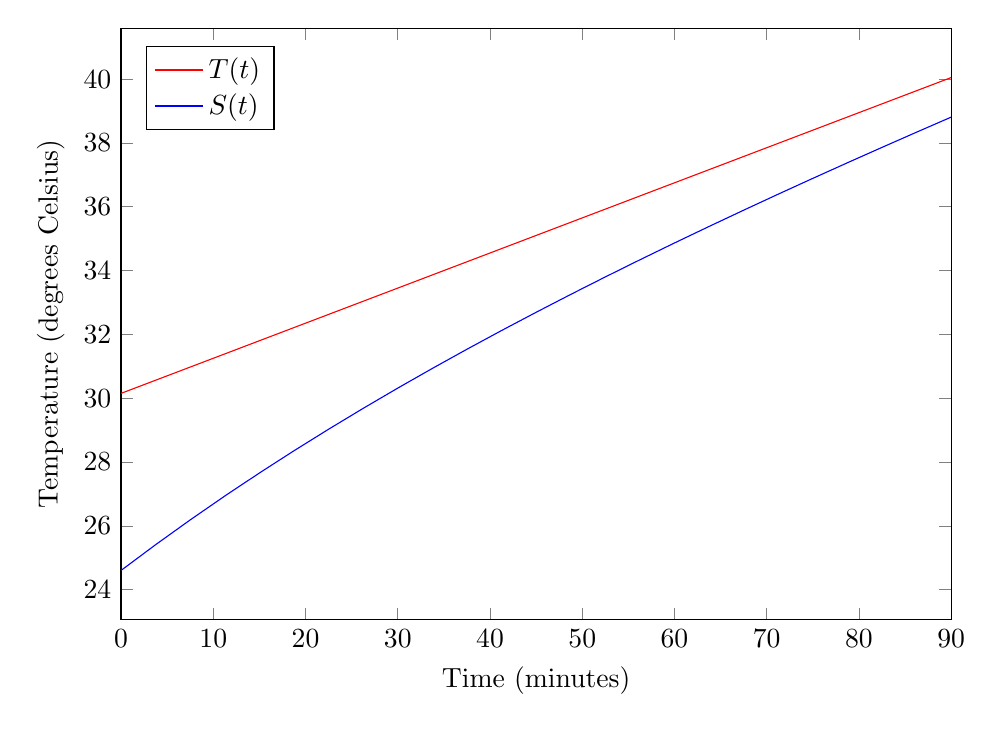
\begin{tikzpicture}
       \begin{axis}
         [width = \textwidth, height=0.75\textwidth, xmin=0, xmax=90, xlabel={Time (minutes)}, ylabel={Temperature (degrees Celsius)}, legend cell align= {left}, legend pos = north west]
         \addplot [color=red, domain=0:90] {0.11*x + 30.15};
         \addlegendentry{\(T(t)\)}
         \addplot [color=blue, domain=0:90] {0.11*x - 5*e^(-0.022*x) + 29.6};
         \addlegendentry{\(S(t)\)}
       \end{axis}
     \end{tikzpicture}
   \end{center}

   Although the snail and the water have different initial temperatures, the model seems to accurately reflect our assumption.
   The rate at which the snail's temperature increases is proportional to the difference between its current temperature and that of the water.
   Thus, as it continues to heat up it does so at a slower rate due to the insulating shell.

   All of our models so far are based on the original assumption that the temperature of the tide pool increases at a constant rate.
   However, this is not necessarily accurate as one considers that Newton's Law of Cooling applies to the environment heating these pools as well.
   The graph of the data points suggests that a logarithmic model for the temperature may have been more accurate.

   Indeed, if we linearize our initial data by taking the logarithm of each time value (omitting \(t = 0\)), we get the following table.
   \begin{center}
     \begin{tabular}{ |c|c| }
       \hline
       \(\ln(t)\) (minutes) & \(T\) (degrees Celsius) \\
       \hline
       1.946 & 31.1 \\
       \hline
       2.485 & 31.9 \\
       \hline
       2.944 & 32.7 \\
       \hline
       3.466 & 34.2 \\
       \hline
       3.611 & 34.7 \\
       \hline
       3.761 & 34.9 \\
       \hline
       3.970 & 35.4 \\
       \hline
       4.094 & 35.8 \\
       \hline
     \end{tabular}
   \end{center}
   Plotting the data, we can obtain a regression line.
   \begin{center}
     \begin{tikzpicture}
       \begin{axis}
         [xlabel={\(\ln(t)\)}, ylabel={\(T\)}, xmin = 1, xmax = 5, grid = both, width = \textwidth, height=0.75\textwidth, legend cell align= {left}, legend pos = north west]

         % Plot data
         \addplot[only marks] table[x=t, y=T] {water_temp_linearized.dat};

         % Plot linear regression
         \addplot[thick, orange]
         table[x = t, y = {create col/linear regression={y=T}}] {water_temp_linearized.dat};

         % Add legend
         \addlegendentry{Data}
         \addlegendentry{
           Linear regression: \(T = \pgfmathprintnumber{\pgfplotstableregressiona} \cdot \ln(t) \pgfmathprintnumber[print sign]{\pgfplotstableregressionb}\)
         };
       \end{axis}
     \end{tikzpicture}
   \end{center}
   Certainly this model has a much stronger correlation with the data set.

   Using this new model, we have a refined model for the temperature of the snail.
   The differential equation formed based on Newton's Law of Cooling becomes
   \begin{equation*}
     \frac{dS}{dt} = k \left( 2.26 \cdot \ln(t) + 26.42 - S \right).
   \end{equation*}
   Note that this is still a linear first order differential equation, so an analytical solution exists and can be found in a similar manner to that used in Section 2.

   If we also remove the assumption that the water's temperature increases indefinitely and suppose that it eventually levels off, we add another level of complexity.
   Stated more formally, we have
   \begin{equation*}
     \lim_{t \to \infty} T(t) = T_{f} < \infty
   \end{equation*}
   In this case, the snail's survival is dependent on \(T_{f}\) being lower than the upper lethal body temperature since the snail's temperature will continue to approach \(T_{f}\) for as long as it remains in the tide pool.
   I believe this restriction implies that both \(T(t)\) and \(S(t)\) are logistic growth functions.
   As a result, their graphs might look like this.
   \begin{center}
     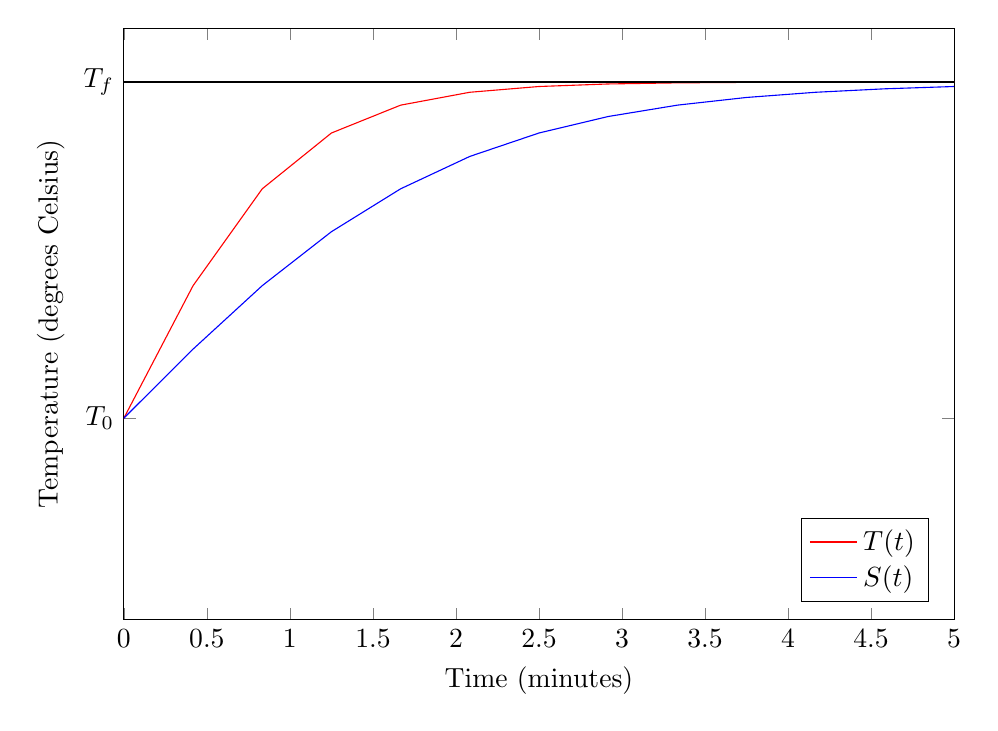
\begin{tikzpicture}
       \begin{axis}
         [xmin = 0, xmax = 5, ymin = 1, xlabel = {Time (minutes)}, ylabel = {Temperature (degrees Celsius)}, width = \textwidth, height=0.75\textwidth, xtick = {},
         ytick = {2.5, 5},
         yticklabels = {\(T_{0}\), \(T_{f}\)},
         legend cell align= {left}, legend pos = south east]



         % Plot two logistic functions
         \addplot[red] {5*(1 + e^-2*x)^-1};
         \addlegendentry{\(T(t)\)};
         \addplot[blue] {5*(1 + e^-1*x)^-1};
         \addlegendentry{\(S(t)\)};
         \addplot[black] {5};
       \end{axis}
     \end{tikzpicture}
   \end{center}
   Note that the graph only displays the right half of the logistic growth model, the idea being that the water's temperature increases less quickly over time and the snail's body temperature increases accordingly.

   \section{Conclusion}
   The approach taken in solving this problem involves forming a model based on given data and using this model to form a differential equation.
   The differential equation is linear and first order, a specific type of equation that we learned how to solve.

   From our study, it is reasonable to conclude that an accurate model of a snail's body temperature in a tide pool factors in the insulation provided by its protective shell.
   Furthermore, it is essential to find an accurate model for how the temperature of the water in the tide pool changes because that is a key term in the differential equation which models the rate of change of the snail's temperature.
   As mentioned in the latter half of the analysis, one heavy limitation in our study is the assumption that the water temperature changes at a constant rate.
   Indeed, it is more reasonable to use a logistic function.
   A more informed claim could be made with a larger data set of times and temperatures in the simulated tide pool.
   Finally, we may still be limited in our differential equation for the temperature of the snail by assuming that the proportion \(k\) is constant.
   It is likely that the snail's body responds to higher body temperatures and attempts to maintain a stable body temperature.
   Thus, the proportion \(k\) is much more likely to be a function of \(S\).
   Although it isn't possible to determine with the given data, it would be plausible to estimate given a dataset measuring how the snail's body temperature changes over time or over various ambient temperatures.



   \begin{thebibliography}{999}
     \bibitem{2924}
      Lisa Driskell; Audrey Malagon (2016), "1-110-S-SnailsInaTidePool,"
      https://www.simiode.org/resources/2924.
   \end{thebibliography}
\end{document}
